\documentclass[12pt]{article}
\usepackage[margin=1in]{geometry}
\usepackage{graphicx}
\usepackage{courier}
\usepackage{times}
\usepackage[T1]{fontenc}
\usepackage{textcomp}
\usepackage{titlesec}
\newcommand{\sectionbreak}{\clearpage}

\graphicspath{ {img/} }

\begin{document}

\begin{titlepage}
  \begin{center}
    \vspace*{1cm}
    \huge\textbf{{Integrating IPv6 into the CPE464 Lab Curriculum}}

    \vspace{1.5cm}

    \begin{figure}[ht!]
      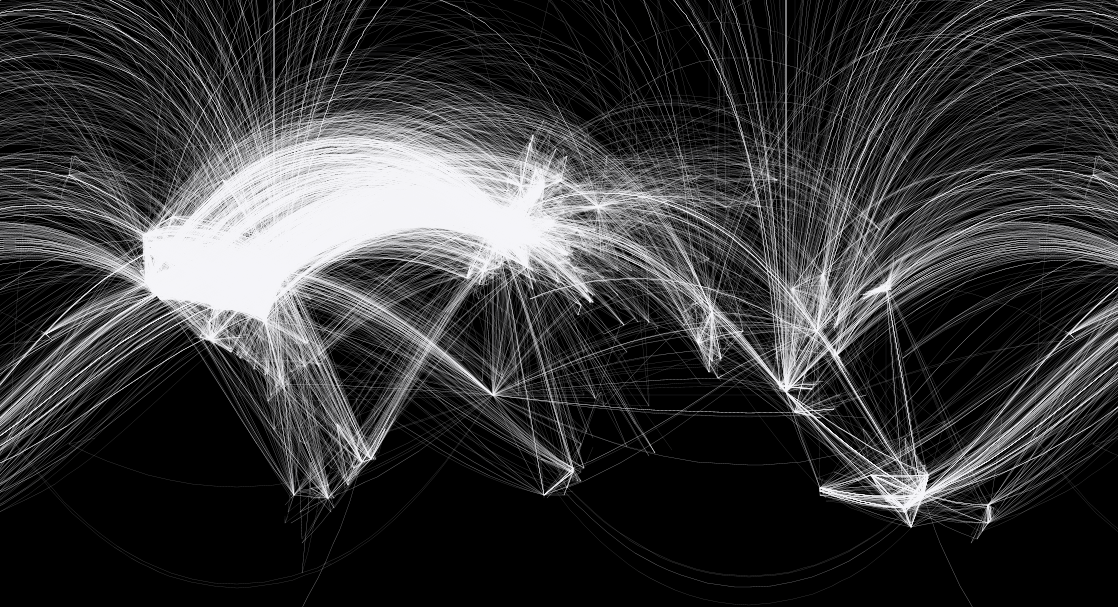
\includegraphics[width=1\textwidth]{internet_map.png}
      \label{fig:internet_map}
    \end{figure}

    \vfill
    \large{
      Jacob Hladky\\
      California Polytechnic State University\\
      San Luis Obispo, CA\\
      \texttt{jhladky@calpoly.edu}
    }

    \vspace{1cm}

    \today   
  \end{center}
\end{titlepage}

\pagenumbering{roman}

\tableofcontents

\listoffigures
\bigskip
\textit{Title Image} \hspace{0.25in} A map of the IPv6 world. The image is a result of mapping the connections between the one hundred thousand most central IPv6 nodes on the Internet.

\listoftables
\clearpage

\pagenumbering{arabic}

\section{Introduction}
The Internet Protocol version 4 was standardized in 1981 by DARPA, a division of the Department of Defense focused on developing cutting-edge technologies. The protocol --- designed to connect every computer on the globe --- could address roughly 4 billion hosts, a number which seemed unbelieveably immense compared to the 200 or so computers on the Internet at the time.\\\\
On the 4th of July of this year the American Registry for Internet Numbers, which assigns Internet addresses (``IP addresses'') is predicted to exhaust its remaining IP addresses. Registries in Asia and Europe have already run out of their share of the ``address space''.  A replacement protocol, version 6, was approved in 1998. The protocol laid dormant for most of the 2000s, but the fast-approaching deadline has spurred its adoption. Figure~\ref{fig:v6_adoption} shows the skyrocketing IPv6 adoption rates. IPv6 is rapidly becoming relevant in both the consumer and enterprise sectors.

\begin{figure}[ht!]
  \centering
  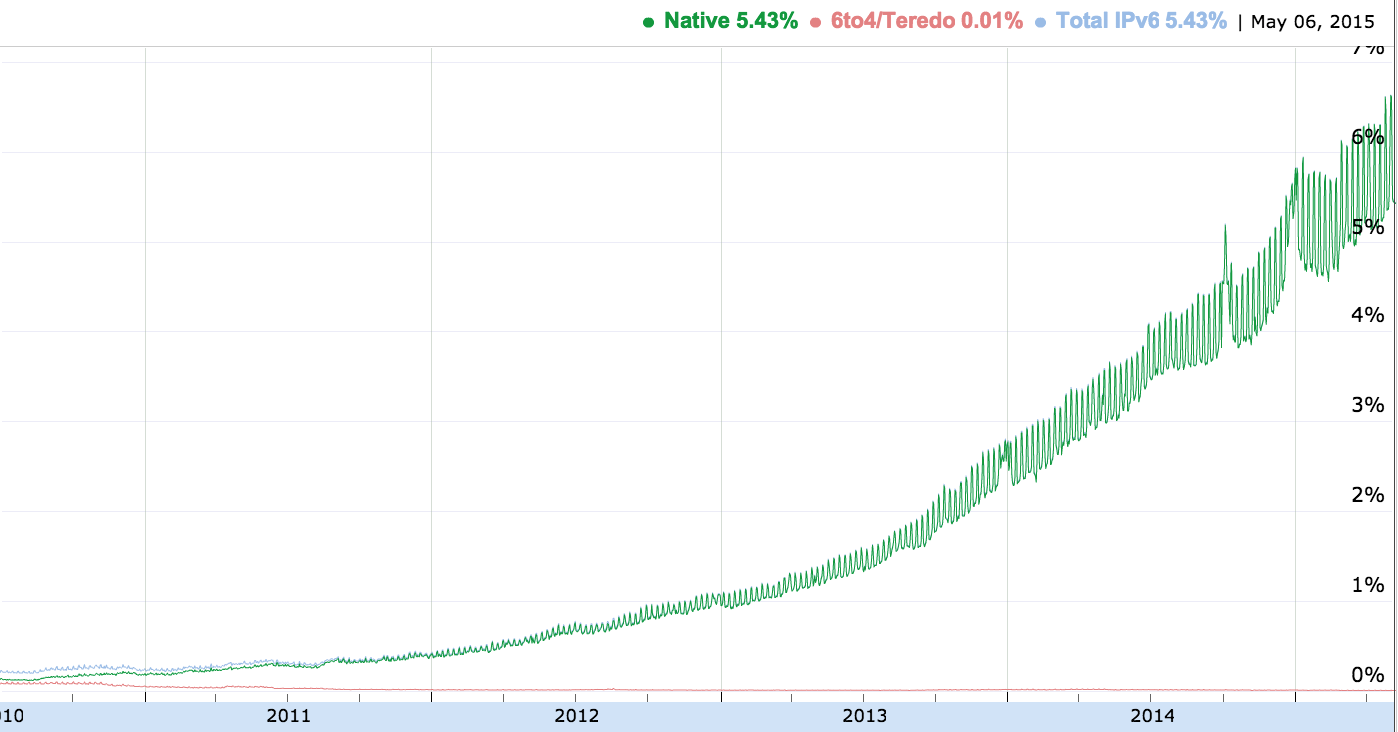
\includegraphics[width=0.75\textwidth]{v6_adoption.png}
  \caption{Percentage of users accessing \texttt{www.google.com} over IPv6}
  \label{fig:v6_adoption}
\end{figure}

\noindent Cal Poly students taking CPE464, Introduction to Computer Networks, will learn IPv4 in depth. In their lab section, which accompanies the lecture, they will implement IPv4 on enterprise-grade networking equipment. The CPE464 lecture will also cover IPv6, but the lab will not. This report will present research about the best way to integrate the teaching of IPv6 into the CPE464 lab curriculum.\\\\
This research can be broken into two parts. The first will address networking technologies that implement IPv6. The second will investigate various ways to integrate these technologies into the existing lab curriculum. This report will then select the optimal option from each and combine them to form a lesson plan, a recommendation on what technology to use and how to use it in the CPE464 lab.\\\\
The \textit{Methods} section of this report will summarize the areas of research that were looked into and what specific sources were researched in those areas. The \textit{Results} section will then present the research findings from each of the methods. The \textit{Conclusion} and \textit{Recommendations} sections will then detail an the best course of action derived from the research. Finally, a \textit{Glossary of Terms} will provide definitions for any unfamiliar terms used in this report.

\section{Methods}
In the course of researching this report I split the problem at hand, of how best to teach the concepts of IPv6 to CPE464 lab students, into two questions. The first: ``What technologies best show how IPv6 is different from IPv4?'' The second: ``What is the best way to integrate these technologies into the CPE464 lab curriculum?'' Correspondingly, I used two different methods of research, using the findings from each method to answer one of the two questions.\\\\
These two questions can be categorized respectively as a technical question and a pedagogical question. To answer the technical question I consulted internet research and to answer the pedagogical question I interviewed Dr. Hugh Smith. These two methods and further detailed in the two subsections below.

\subsection{Interview with Dr. Hugh Smith}
interview blah blah blah


IN MY RESULTS I WILL DISCUSS THE PEDAGOGICAL METHODS HERE... NOT A LOT OF RESEARCH FOR THIS SECTION
THIS IS THE CORE FOR THE PEDAGOGICAL SECTION


\subsection{Secondary Research}
blah blah explanation of secondary research


\subsubsection{Cisco: ``IPv6 Tunnel though a IPv4 Network''}
tunneling blahl blah  THIS IS ONE OF THE TECHNICAL METHODS


\subsubsection{Cisco: ``IPv6 Autoconfiguration''}
dhcp... THIS IS ANOTHER OF THE TECHNICAL METHODS


\subsubsection{CircleID: ``DHCP for IPv4 vs. IPv6''}
NEED A THIRD, OKAY, THAT WILL BE THIS THING HERE...

\subsubsection{Cisco: ``RIP for IPv6''}


aaaa

\section{Results}
% the results will follow the same structure as the methods, but i will just present conclusions

\subsection{Interview with Dr. Hugh Smith}
adsfadsf
\subsection{Cisco: ``IPv6 Tunnel though a IPv4 Network''}
asdfasdf
\subsection{Cisco: ``IPv6 Autoconfiguration''}
dsfadsf
\subsection{CircleID: ``DHCP for IPv4 vs. IPv6''}
aaaaa
\subsection{Cisco: ``RIP for IPv6''}
aaaa

\section{Conclusions}
aaaa

\section{Recommendations}
aaaa

\section{Glossary of Terms}
aaaa

\section{Works Cited}
aaaa

\end{document}



